\subsection{Advertisement Counter}
Advertising platforms need to accurately record impressions and clicks, in order to analyse advertising data. They use distributed counters, which are challenging to implement in a dynamic, fault-prone environment. \gls{crdt} counters are a promising solution; the challenge is to scale to an extreme numbers of users.

Rovio's Ads service keeps track of impressions and clicks for ads per campaign/ad/country. Typically these counts have some upper bounds after which the ad should not be shown any more. The upper bound may consist of the sum of several counters (e.g show the same ad 50,000 times in the US, 10,000 times in the UK and 100,000 times in total), so it is not really feasible to enforce the upper bound on the data storage layer.

The main use for the tracking data is to control the rate of ads shown to the users. The campaign capacity should be spread evenly over the duration of the campaign instead of showing all the impressions during the first hour of the campaign. Therefore, the data must be updated in real time although a good estimate is normally enough. 


\subsubsection{Current Implementation}
The system maybe represented by the various constants and variables that follow, Table \ref{tab:ads_constants_variables}.
\begin{table}[!ht]
	\begin{tabular}{|p{0.7cm}|p{5.8cm}|r| }
		\hline
			\multicolumn{1}{|c|}{Name} & \multicolumn{1}{c|}{Description} & \multicolumn{1}{c|}{Type} \\
		\hline
		\hline
			$DC$ & It is the set of all \glspl{dc}. $d$ identifies one of the \glspl{dc}, $d \in \{1,\dots, |DC|\}$. & $\mathbb{Z}_{+} $\\
		\hline
			$AD$ & It is the set of all advertisement-campaigns. $a$ identify one of the ads, $a \in \{1,\dots, |AD|\}$. & $\mathbb{Z}_{+}$ \\
		\hline
			$DV$ & It is the set of devices. $dv$ represents one of those devices, $dv \in \{1,\dots, |DV|\}$. & $\mathbb{Z}_{+}$ \\
		\hline
			$Nodes$ & It is the set of nodes. $n$ represents one of those nodes, $n \in \{1,\dots, |Nodes|\}$. & $\mathbb{Z}_{+}$ \\
		\hline
	\end{tabular}
	\vspace{.1cm}

	\begin{tabular}{|p{7cm}|p{.2cm}| }
		\hline
			Name/Description & \multicolumn{1}{c|}{Type} \\
		\hline
		\hline
			$T_{a}, T^{start}_{a}, T^{end}_{a}$ & $\mathbb{R}_{+}$ \\
		\hline
			 \multicolumn{2}{|p{7.1cm}|}{$T_{a}$ is the duration of the campaign for ad $a$.
			$T^{start}_{a}$ represents the beginning of the campaign and $T^{end}_{a}$ the end, with $T_{a}= T^{start}_{a} - T^{end}_{a}$.}\\
		\hline
		\hline
			$maxTotalViews(a)$ & $\mathbb{Z}_{+}$ \\
		\hline
			\multicolumn{2}{|p{7.1cm}|}{It is the maximum total number of times the ad $a$ should be shown.} \\
		\hline
		\hline
			$maxTotalViewsPerDC(a, d)$ & $\mathbb{Z}_{+}$ \\
		\hline
			 \multicolumn{2}{|p{7.1cm}|}{It is the total number of times the ad $a$ should be shown by \gls{dc} $d$.} \\
		\hline
		\hline
			$maxViewsPerDevice(a)$ & $\mathbb{Z}_{+}$ \\
		\hline
			\multicolumn{2}{|p{7.1cm}|}{It represents the maximum number of times the ad $a$ should be presented on a device.} \\
		\hline
		\hline
			$viewsPerDevice(a, dv)$ & $\mathbb{Z}_{+}$ \\
		\hline
			\multicolumn{2}{|p{7.1cm}|}{It is the number of times the ad $a$ has been shown on the device $g$. $h(t)_{ag}$ is the same than $h_{ag}$.} \\
		\hline
		\hline
			$verifiedViews(a, n, q)$ & $\mathbb{Z}_{+}$ \\
		\hline
			\multicolumn{2}{|p{7.1cm}|}{It is the verified number of times an ad $a$ has been shown by node $q$ as the node $n$ report it, $n, q \in \{1,\dots, |Nodes|\}$.} \\
		\hline
		\hline
			$averageViews(a)$ & $\mathbb{Z}_{+}$ \\
		\hline
			\multicolumn{2}{|p{8.1cm}|}{It is the average number of times ad $a$ is shown. The workload is equally spread between all the nodes, $\frac{averageViews(a)}{|Nodes|}$.} \\
		\hline
	\end{tabular}

	\caption{Ad Counters Constants and Variables.}
	\label{tab:ads_constants_variables}
\end{table}

Equality \ref{eq:ad_spread} states that the total maximum number of times an ad should be presented in each \gls{dc} is equal to  the maximum total number of times that ad should be shown in the campaign, and Inequality \ref{eq:total_device_ads} states that the ad $a$ must be shown on any device only a maximum number of times of $maxTotalViews(a)$. The total number of times that ad $a$ has been shown on completion of the campaign is expressed by Equation \ref{eq:real_total_ads}. The goal of the system is to minimise $\Delta_{a}$, $\Delta_{a} \in \mathbb{N}_{0}$.
\begin{equation} \label{eq:ad_spread}
	maxTotalViews(a) = \sum_{d \in DC} maxTotalViewsPerDC(a, d)
\end{equation}
\begin{equation} \label{eq:total_device_ads}
	maxViewsPerDevice(a) \ge viewsPerDevice(a, dv)
\end{equation}
\begin{multline} \label{eq:real_total_ads}
	maxTotalViews(a) = \sum_{dv \in DV} viewsPerDevice(a, dv) + \Delta_{a}\\ \forall ~  t \ge T^{end}_{a}
\end{multline}

The Ads service runs on multiple service nodes, so in order to avoid write conflicts each of those nodes has its own document for the impression and click counters in Riak. This is already a simplified implementation of the counter \gls{crdt}. The true value of the counter can be obtained by calculating the sum of all counters manually.

Even if the current solution works, it is neither very elegant nor easy to maintain. The \gls{crdt} counters will provide a more efficient solution for updating the counters. The ad system does not need a strict limit for the counter and we can implement an optimistic solution: if the counter value is less than the limit then show the ad and increase the counter. This may result in showing the ad too many times, but it is \textquotedbl{}close enough\textquotedbl{}. Client applications running on different kinds of devices (mobile phones, tablets, etc.) connect to the Ads service in order to determine which ads to show to their users. The same ad should not be shown on the same device any more than 3 times a day ($maxViewsPerDevice(a, dv) = 3$), so the Ads service keeps track of on which device has been shown which ad and when. This data is currently stored in one document that contains information on the ads shown on a device during the last couple of days (basically which ad has been shown and when). It might be possible to utilise \glspl{crdt} in this document.
%, but the current implementation has no major issues, either.

In a \gls{dc} each server node has its own cache representing the counters. The cache could be dropped theoretically, but in practice it will be needed. The counters get synced between the life statistics nodes via Riak. Each counter will have some copies, e.g. three, on the database meaning the value is formed based on those copies. The average number of times, ad $a$ is shown, is $averageViews(a)$  for an interval of time, so the estimated number of times the ad $a$ has been shown is represented by Equation \ref{eq:dc_counter} as seen by node $n$, note that only one \gls{dc} is currently used. Also the verified number of times an ad has been shown, $ verifiedViews(a, n)$, is the number of times node $n$ reported to have shown the ad $a$ in the last synchronisation at previous period of time.
\begin{multline} \label{eq:dc_counter}
	views(a, n) = \sum_{q \in Nodes}  verifiedViews(a, n, q)\\ + averageViews(a)
\end{multline}

The sum of all the times an ad $a$ has been seen corresponds to the real number of times the ad $a$ has been shown by the system, as shown by Equation \ref{eq:real_dc_counter}. The total number os times the ad $a$ has been seen at any time, $views(a, n)$, as seen by a node $n$ may be less or equal to the real total number of times the ad $a$ has been shown, $views(a)$, as shown by Inequality \ref{eq:compare_dc_counters}. This inequality should be eventually (after last synchronisation) an equality.
\begin{equation} \label{eq:real_dc_counter}
	views(a) = \sum_{n \in Nodes}  verifiedViews(a, n, n)
\end{equation}
\begin{equation} \label{eq:compare_dc_counters}
	views(a) \ge views(a, n)
\end{equation}

Also the numbers of times an ad $a$ has been shown after the ad-campaign has concluded must be the same irrespective of the node reporting it, as shown by Equation \ref{eq:dc_counter_per_node}.
\begin{multline} \label{eq:dc_counter_per_node}
	views(a) = views(a, n) = views(a, m)\\ \forall ~ n, m \in \{1,\dots, |Nodes|\}, t \ge T^{end}_{a} + \Delta t
\end{multline}

The life statistics nodes serve the entire state of all campaigns. They hold a cache for the data and keep it in sync via Riak. There is a local estimation in place between the nodes synchronisation since the data is not synced on every update they get from the ad servers.


\subsubsection{Multiple Data Centres}
The campaign counter could also be spread throughout the different \glspl{dc} in each country which will improve the accuracy of the counter, Figure \ref{fig:ads_countert_}. At each \gls{dc} a part of the overall counter would be assigned to each \gls{dc}, which will only be able to service this number of times the specific ad. The changes to the ad counters are replicated in the other \glspl{dc} at different intervals.
\begin{figure}[ht!]
	\centering
	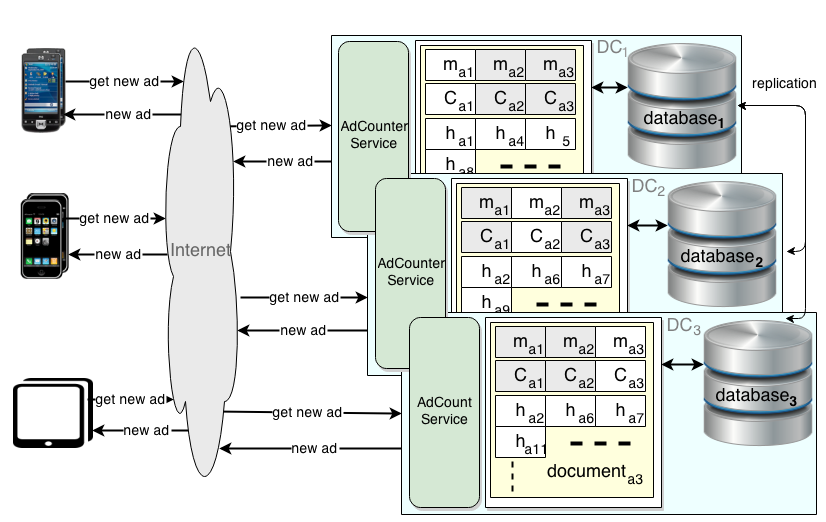
\includegraphics[width=1\linewidth]{figures/AdsServiceSpread2DCs.png}

	\caption{Overview for the distribution of counters with three \glspl{dc}, $|DC| = 3$.}
	\label{fig:ads_countert_}
\end{figure}

The distribution of the counter could be based on different criterion, e.g. population size covered by each \gls{dc}, existing statistics from previous campaigns or studies, costumer preferences, intention of the campaign like the increase in the market share in an already established part of the territory or entering a new area to extend the territory covered.

It may be decided that when a device serviced by a \gls{dc} changes to be serviced by another \gls{dc}, e.g. by changing location, then its counter is now know by the new servicing \gls{dc}, potentially showing those ads already seen again, otherwise the device counter needs to be replicated between \glspl{dc}, but not necessarily to all \glspl{dc}.

The extra constants required for multiple \glspl{dc} are presented below, Table \ref{tab:ads_extra_constants_variables}.
\begin{table}[!ht]
	\begin{tabular}{|p{6.5cm}|p{.2cm}|}
		\hline
			Name/Description & \multicolumn{1}{c|}{Type} \\
		\hline
		\hline
			$Nodes_{d}$ & $\mathbb{Z}_{+}$ \\
		\hline
			\multicolumn{2}{|p{8.1cm}|}{It is the set of nodes in \gls{dc} $d$. $n$ represents one of those nodes, $n \in \{1,\dots, |Nodes_{d}|\}$.} \\
		\hline
		\hline
			$averageViews(a, d)$ & $\mathbb{Z}_{+}$ \\
		\hline
			\multicolumn{2}{|p{8.1cm}|}{It is the average number of times ad $a$ is shown for a given time interval by \gls{dc} $d$. The workload is equally spread between all the nodes in the same \gls{dc}, $\frac{averageViews(a, d)}{|Nodes_{d}|}$.} \\
		\hline
		\hline
			$verifiedViews(a, d, n)$ & $\mathbb{Z}_{+}$ \\
		\hline
			\multicolumn{2}{|p{8.1cm}|}{It is the verified number of times an ad $a$ has been shown by node $n$ in \gls{dc} $d$ as the node $n$ reported to have shown the ad $a$ in the last synchronisation at previous period of time.} \\
		\hline
		\hline
			$targerMaxViews(a, d)$ & $\mathbb{Z}_{+}$ \\
		\hline
			\multicolumn{2}{|p{8.1cm}|}{It is the maximum number of times the ad $a$ should be shown by \gls{dc} $d$. This may as well be used to restrict the locations (represented by $L$), e.g. country an ad is shown. \glspl{dc} outside these locations will not show the ad so $targerMaxViews(a, d) = 0 ~ \forall ~ a \not\in L$. Also the replication will only be necessary between the \glspl{dc} with $targerMaxViews(a, d) > 0$.} \\
		\hline
		\hline
			$views(a, d)$ & $\mathbb{N}_{0}$ \\
		\hline
			\multicolumn{2}{|p{8.1cm}|}{It is the total number of times the ad $a$ has been shown on devices by \gls{dc} $d$ from the beginning of the campaign, $T^{start}_{a}$, to time $t$.} \\
		\hline
		\hline
			$totalViews(a)$ & $\mathbb{Z}_{+}$ \\
		\hline
			\multicolumn{2}{|p{8.1cm}|}{It is the overall total number of times the ad $a$ has been shown from the beginning of the campaign, $T^{start}_{a}$, to time t.} \\
		\hline
	\end{tabular}

	\caption{Ad Counters extra Constants and Variable.}
	\label{tab:ads_extra_constants_variables}
\end{table}

The model needs to be extended by the following expressions:
\begin{equation} \label{eq:dcs_counter_limit}
	targetMaxViews(a, d) \ge views(a, d)
\end{equation}
\begin{equation} \label{eq:dcs_counter_start}
	views(a, d) = 0 ~ \forall ~ t \le T^{start}_{a}
\end{equation}
\begin{equation} \label{eq:dcs_counter_final}
	targetMaxViews(a, d) =  views(a, d) ~ \forall ~ t \ge T^{end}_{a}
\end{equation}
\begin{equation} \label{eq:total_ads}
	totalMaxView(a)  = \sum_{d \in DC} targetMaxViews(a, d)
\end{equation}
\begin{equation} \label{eq:total_ads_at_time_t}
	totalViews(a) =  \sum_{d \in DC} views(a, d)
\end{equation}
Inequality \ref{eq:dcs_counter_limit} states that the counter $views(a, d)$ always has a limit which it is the maximum number of times the ad $d$ must be shown by \gls{dc} $d$, whereas at the beginning of the campaign no ads has been shown as stated by Equation \ref{eq:dcs_counter_start}, and once the campaign has finish the total number of times an ad has been shown by each \gls{dc} is the same than the maximum allowed as expressed by Equation \ref{eq:dcs_counter_final}. Equation \ref{eq:total_ads} states that the ads are distributed through out all the \glspl{dc}. Equation \ref{eq:total_ads_at_time_t} states that the overall total number of times an ad $a$ has been shown is equal to the sum of the number of times the ad $a$ has been shown by each \gls{dc}.

\begin{equation} \label{eq:total_ads2}
	maxTotalViews(a) \ge \sum_{d \in DC} totalViews(a, d)
\end{equation}
\begin{equation} \label{eq:total_ads3}
	maxTotalViews(a) = totalViews(a) + \Delta_{a} ~ \forall ~ t \ge T^{end}_{a}
\end{equation}
Inequality \ref{eq:total_ads2} gives the total limit for all the $totalViews(a, d)$ which can be obtained from Inequality \ref{eq:dcs_counter_limit} and Equation \ref{eq:total_ads}, whereas Equation \ref{eq:total_ads3} shows that the total number of times ad $a$ has been shown, once the campaign has concluded $t \ge T$, is equal to the total number ad $a$ should has been shown.

Also Equation \ref{eq:dc_counter} can be generalised for many \glspl{dc} as shown in Equation \ref{eq:dc_total_counter}.
\begin{multline} \label{eq:dc_total_counter}
	views(a, d) = \sum_{n \in Nodes_{d}}  verifiedViews(a, d, n) +\\ averageViews(a, d)
\end{multline}

There is the possibility that a device in the border between two \glspl{dc}, where the ad is run, receives more than its limit if the two \glspl{dc} are out of sync for that device.

To have into account the state of the data in each of the \glspl{dc} the previous definitions are extended and some new introduced below, Table \ref{tab:ads_entended_constants_variables}.
\begin{table}[!ht]
	\begin{tabular}{|p{6.5cm}|p{.2cm}| }
		\hline
			Name/Description & \multicolumn{1}{c|}{Type} \\
		\hline
		\hline
			 $views(a, d, q)$ & $\mathbb{Z}_{+}$ \\
		\hline
			\multicolumn{2}{|p{8.1cm}|}{It is the total number of times the ad $a$ has been shown on devices by \gls{dc} $d$ from the beginning of the campaign to time $t$ as it is seen by \gls{dc} $q$, $d, q \in \{1,\dots, |DC|\}$.}  \\
		\hline
		\hline
			 $\Delta views(a, d, q)$ & $\mathbb{Z}_{+}$ \\
		\hline
			 \multicolumn{2}{|p{8.1cm}|}{It is the discrepancy of the total number of times the ad $a$ has been shown on devices by \gls{dc} $d$ from the beginning of the campaign to time $t$ as reported by \gls{dc} $q$, as it is represented in Equation \ref{eq:dc_counter_diff}.} \\
		\hline
		\hline
			 $\Delta totalViewsDiscrepancy(a, d, q)$ & $\mathbb{Z}_{+}$ \\
		\hline
			\multicolumn{2}{|p{8.1cm}|}{It is the absolute total discrepancy of the overall total number of times the ad $a$ has been shown from the beginning of the campaign to time t when using the values provided by \gls{dc} $d$, which it is represented in Equation \ref{eq:dc_total_counter_diff}.} \\
		\hline
	\end{tabular}
	
	\caption{Ad Counters Constants and Variable for discrepancies in values between \glspl{dc}.}
	\label{tab:ads_entended_constants_variables}
\end{table}
The discrepancy of the counter for ad $a$ shown on devices by \gls{dc} $d$ is zero when it is reported by the same \gls{dc} as expressed in Equation \ref{eq:dc_counter_own_diff}.
\begin{equation} \label{eq:dc_counter_diff}
	\Delta views(a, d, q) = views(a, d, d) - views(a, d, q)
\end{equation}
\begin{equation} \label{eq:dc_counter_own_diff}
	\Delta views(a, d, d) = 0
\end{equation}
\begin{equation} \label{eq:dc_total_counter_diff}
	\Delta totalViewsDiscrepancy(a, d) = \sum_{q \in DC} \mid \Delta views(a, d, q) \mid
\end{equation}

The total counter is said to be consistent throughout all the \glspl{dc} if there is not any discrepancy between all the \glspl{dc}, as expressed in Equation \ref{eq:dc_total_counter}.
\begin{equation} \label{eq:dc_total_counter_coherent}
	\Delta totalViewsDiscrepancy(a, d) = 0
\end{equation}
